\documentclass[../../General.tex]{subfiles}
\begin{document}

\section{Diseño de subsistema de orientación de piranómetro}

\subsection{Descripción general del subsistema}

El subsistema de orientación, mostrado en la Figura \ref{fig:SubsistemaOrientacionCAD}, ejecuta el giro de alabeo (\textit{roll}) de la plataforma que porta el piranómetro. El eje de giro es paralelo a la dirección de avance del robot; de este modo, cuando el robot circula por el pasillo paralelo a las filas de módulos, el giro de alabeo permite igualar la inclinación del sensor con la del plano de los módulos fotovoltaicos. Para sistemas de monitoreo Clase A, la norma IEC 61724-1 exige que los sensores de irradiancia alineados con el plano de los módulos mantengan una tolerancia de $0.5^\circ$ en inclinación y de $1.0^\circ$ en azimut \citep{IEC61724-1_2021}. Este subsistema controla la inclinación; la tolerancia de azimut depende del rumbo del robot respecto a la fila de módulos y no se controla con este subsistema.

El subsistema se monta sobre el de elevación (Sección \ref{sec:subsistema_elevacion}): una viga 2040 del subsistema de orientación se dispone en sentido longitudinal, paralela al avance, y se fija al alma de la pieza en U del subsistema de elevación. El motor NEMA 17 y la caja del tornillo sin fin quedan hacia el frente del robot.

El control de este subsistema corrige únicamente la inclinación lateral (\textit{roll}); no corrige el cabeceo (\textit{pitch}). Como el paralelogramo de elevación traslada la plataforma sin rotarla, el \textit{pitch} del sensor es el del chasis. Por ello, la medición se realiza solo en tramos casi planos. El MPU-6050 montado en el eje basculante mide el vector gravedad en tres ejes, de modo que entrega tanto el \textit{roll} como el \textit{pitch} de la plataforma, y es la medición más directa para verificar esa condición.

Para una plataforma inclinada un ángulo $\beta$ alrededor del eje longitudinal, un \textit{pitch} $p$ desvía el azimut de la normal del sensor en $p \cot\beta$ aproximadamente. Con la tolerancia de azimut de $1.0^\circ$ de la IEC 61724-1, el \textit{pitch} admisible es $|p| \leq 1.0^\circ \cdot \tan\beta$, cuyos valores se muestran en la Tabla \ref{tab:pitch_admisible_tilt}. Este límite asigna toda la tolerancia de azimut al \textit{pitch}, es decir, supone que el rumbo del robot es paralelo a la fila de módulos. Si el rumbo se desvía, ese error consume parte de la misma tolerancia y el \textit{pitch} admisible se reduce en la misma proporción.

\begin{center}
    \footnotesize
    \begin{xltabular}{0.8\textwidth}{|>{\centering\arraybackslash}X|>{\centering\arraybackslash}X|>{\centering\arraybackslash}X|}
        \caption{\textit{Pitch} admisible según la inclinación de la plataforma\label{tab:pitch_admisible_tilt}} \\
        \hline
        \rowcolor[HTML]{D9E1F2}
        Inclinación $\beta$ & \textit{Pitch} admisible [$^\circ$] & ¿Cumple $\geq 0.2^\circ$? \\ \hline
        \endfirsthead

        \multicolumn{3}{c}%
        {\tablename\ \thetable{} -- Continuación de la página anterior} \\
        \hline
        \rowcolor[HTML]{D9E1F2}
        Inclinación $\beta$ & \textit{Pitch} admisible [$^\circ$] & ¿Cumple $\geq 0.2^\circ$? \\ \hline
        \endhead

        \hline
        \endfoot

        \hline
        \endlastfoot

        $5^\circ$ & $0.087$ & No \\ \hline
        $10^\circ$ & $0.18$ & No \\ \hline
        $12^\circ$ & $0.21$ & Sí ($\beta_{\min}$) \\ \hline
        $18^\circ$ & $0.32$ & Sí \\ \hline
        $30^\circ$ & $0.58$ & Sí \\ \hline
    \end{xltabular}
\end{center}

El límite de \textit{pitch} solo es verificable si supera la incertidumbre con la que se mide. Con la exactitud de $0.1^\circ$ del MPU-6050 tras la calibración de seis posiciones y la compensación de temperatura y un margen de 2, se exige $1.0^\circ \cdot \tan\beta \geq 0.2^\circ$, lo que da $\beta_{\min} = 11.3^\circ$, que se redondea a $\beta_{\min} = 12^\circ$. Para $\beta \geq 12^\circ$, el subsistema cumple la tolerancia de inclinación y la de azimut de la norma, siempre que el \textit{pitch} del chasis no supere el valor de la Tabla \ref{tab:pitch_admisible_tilt}. Para $\beta < 12^\circ$, solo se verifica la tolerancia de inclinación de $0.5^\circ$ y no se reclama la de azimut. La IEC 61724-1 exige nivelar los sensores de irradiancia global horizontal dentro de $0.5^\circ$ sin fijarles tolerancia de azimut, y, para los sensores en el plano de los módulos montados en una estructura independiente de ellos, establece que, si no puede lograrse la alineación, el error de alineación debe medirse y documentarse \citep{IEC61724-1_2021}. Por ello, para $\beta < 12^\circ$ el robot registra con cada medición el \textit{pitch} que mide el MPU-6050, del que se obtiene el error de azimut $p \cot\beta$. El umbral no excluye ninguna inclinación de módulo: solo define si se reclama la tolerancia de azimut o se documenta el error. El margen de 2 y el umbral de $12^\circ$ son criterios de diseño de este trabajo, no valores de la norma. El rango mecánico de $\pm 30^\circ$ no cambia.

El giro se transmite desde un motor a pasos NEMA 17 mediante un tornillo sin fin y una corona, que se fabrican en torno CNC. La transmisión se autobloquea en reposo, de modo que el peso del sensor y la carga de viento no hacen retroceder el mecanismo. Un sensor inercial MPU-6050, montado en una chapa solidaria al eje, mide el ángulo de alabeo y cierra el lazo de control de posición.

\begin{figure}[H]
	\captionsetup{justification=raggedright, singlelinecheck=false, labelsep=none}
	\caption[Vista isométrica y derecha del subsistema de orientación.]{}
	\textit{Vista isométrica y derecha del subsistema de orientación.} \par\medskip

	\begin{minipage}{0.5\textwidth}
		\centering
		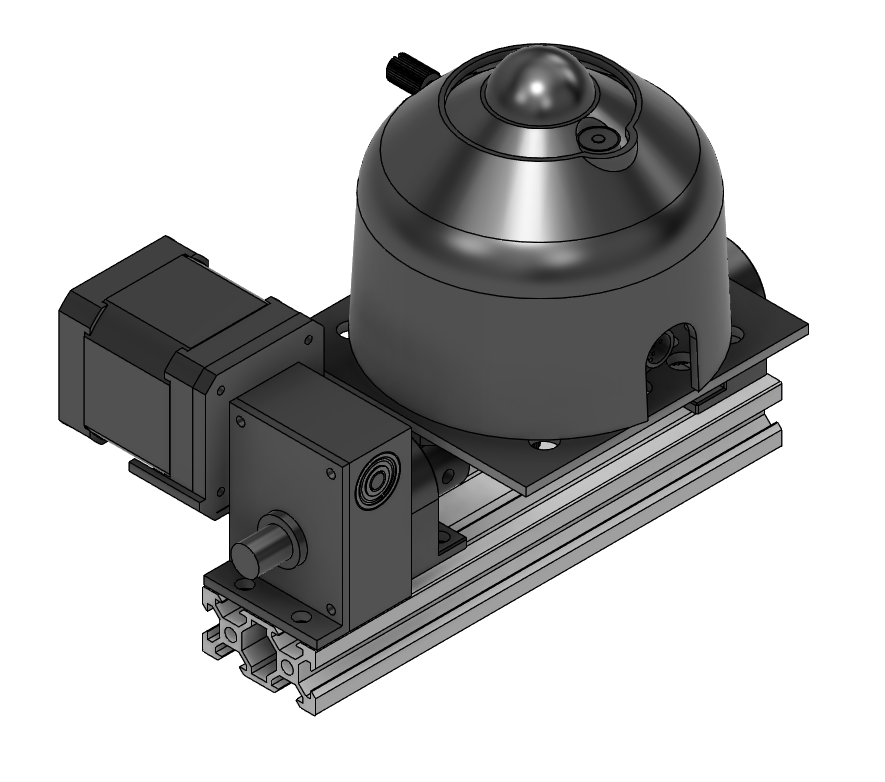
\includegraphics[width=\linewidth]{Recursos/Imagenes/ImagenesDisenoMecanico/MECANISMO_ORIENTACION_ISO1.png}
	\end{minipage}\hfill
	\begin{minipage}{0.5\textwidth}
		\centering
		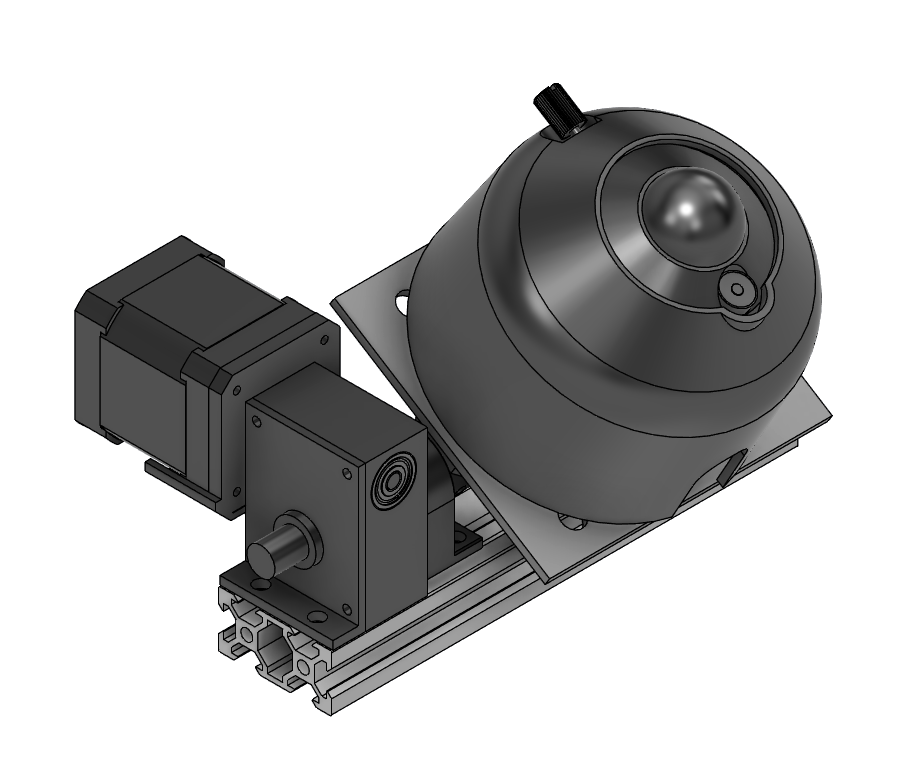
\includegraphics[width=\linewidth]{Recursos/Imagenes/ImagenesDisenoMecanico/MECANISMO_ORIENTACION_ISO2.png}
	\end{minipage}
	\par\medskip

	\raggedright
	\footnotesize \textit{Nota.} Elaboración propia.
	\label{fig:SubsistemaOrientacionCAD}
\end{figure}

\subsection{Planteamiento inicial y parámetros de diseño}

El subsistema debe orientar una plataforma que gira alrededor de un eje central y que soporta el sensor de irradiancia. El diseño debe sostener la carga en cualquier punto de la trayectoria, resistir la carga de viento y alcanzar la tolerancia angular de la norma. Los datos de entrada y las restricciones del análisis se resumen en la Tabla \ref{tab:parametros_diseno_tilt}.

\begin{center}
    \footnotesize
    \begin{xltabular}{\textwidth}{|p{3.5cm}|>{\centering\arraybackslash}p{2.2cm}|>{\centering\arraybackslash}p{2.8cm}|>{\centering\arraybackslash}X|}
        \caption{Datos de entrada y restricciones del subsistema de orientación\label{tab:parametros_diseno_tilt}} \\
        \hline
        \rowcolor[HTML]{D9E1F2}
        Parámetro & Símbolo & Valor & Descripción \\ \hline
        \endfirsthead

        \multicolumn{4}{c}%
        {\tablename\ \thetable{} -- Continuación de la página anterior} \\
        \hline
        \rowcolor[HTML]{D9E1F2}
        Parámetro & Símbolo & Valor & Descripción \\ \hline
        \endhead

        \hline
        \endfoot

        \hline
        \endlastfoot

        \multicolumn{4}{|l|}{\textbf{Carga y plataforma}} \\ \hline
        Masa de diseño del sensor & $m_{\text{carga}}$ & $0.50\text{ kg}$ & Envolvente de piranómetros Clase A de masa $\leq 0.50\text{ kg}$. \\ \hline
        Excentricidad horizontal del centro de masa & $d_{\text{cm}}$ & $25\text{ mm}$ & Distancia horizontal supuesta, con la plataforma nivelada, entre el eje de giro y el centro de masa del sensor. \\ \hline
        Altura del centro de masa del sensor & $z_{s}$ & $54.3\text{ mm}$ & Distancia vertical, con la plataforma nivelada, entre el eje de giro y el centro de masa del sensor, medida en el modelo CAD. \\ \hline
        Masa de la plataforma & $m_{\text{plat}}$ & $0.25\text{ kg}$ & Plataforma, soportes y elementos de sujeción. En el modelo CAD, la placa de aluminio y su tornillería suman $0.066\text{ kg}$; los soportes, impresos en ABS, no se cuentan. \\ \hline
        Altura del centro de masa de la plataforma & $z_{p}$ & $16.4\text{ mm}$ & Distancia vertical entre el eje de giro y el centro de masa de la placa y su tornillería, medida en el modelo CAD. \\ \hline
        Longitud de la plataforma & $L_{\text{plat}}$ & $90\text{ mm}$ & Dimensión de la plataforma en el plano de giro. La placa mide $90\times100\times3\text{ mm}$; los $100\text{ mm}$ van a lo largo del eje basculante. \\ \hline
        \multicolumn{4}{|l|}{\textbf{Movimiento}} \\ \hline
        Rango angular & $\theta$ & $-30^\circ$ a $+30^\circ$ & Barrido total $\Delta\theta = 60^\circ$. \\ \hline
        Tiempo de barrido & $t_{b}$ & $5.0\text{ s}$ & Tiempo para recorrer el barrido completo. \\ \hline
        Fracción de aceleración & $f_{a}$ & $0.25$ & Fracción de $t_b$ en aceleración e igual en desaceleración. \\ \hline
        Tolerancia de inclinación & $\varepsilon_{\text{adm}}$ & $0.5^\circ$ & IEC 61724-1, Clase A \citep{IEC61724-1_2021}. \\ \hline
        \multicolumn{4}{|l|}{\textbf{Transmisión}} \\ \hline
        Módulo axial & $m$ & $1.0\text{ mm}$ & Módulo del par tornillo sin fin y corona. \\ \hline
        Entradas del sin fin & $Z_1$ & $1$ & Número de hilos del tornillo sin fin. \\ \hline
        Dientes de la corona & $Z_2$ & $30$ & Relación de reducción $i = 30$. \\ \hline
        Diámetro exterior del sin fin & $d_{\text{ext}}$ & $14.5\text{ mm}$ & Diámetro de paso $d_w = d_{\text{ext}} - 2m = 12.5\text{ mm}$. \\ \hline
        Ángulo de presión normal & $\phi_n$ & $20^\circ$ & Valor de los pares de módulo axial de KHK \citep{khk_gear_ref}. \\ \hline
        Coeficiente de fricción & $\mu_s$ & $0.15$ & Fricción estática acero--bronce lubricado. \\ \hline
        Juego circunferencial & $j_t$ & $0.28\text{ mm}$ & Referencia de transmisiones comerciales de igual módulo y número de dientes. \\ \hline
        \multicolumn{4}{|l|}{\textbf{Viento (NTE E.020)}} \\ \hline
        Velocidad de diseño & $V$ & $75\text{ km/h}$ & Valor mínimo normativo a $10\text{ m}$ de altura. \\ \hline
        Factor de forma & $C$ & $1.5$ & Elemento con una dimensión corta en la dirección del viento. \\ \hline
        Factor de ráfaga & $f_r$ & $1.2$ & Estructura Tipo 2. \\ \hline
        Área expuesta & $A_{\text{exp}}$ & $0.012\text{ m}^2$ & Envolvente del área proyectada del sensor y la plataforma. El modelo CAD da entre $0.0078$ y $0.0089\text{ m}^2$. \\ \hline
        Brazo del centro de presión & $h_{\text{cp}}$ & $60\text{ mm}$ & Envolvente de la distancia del centro de presión al eje de giro. El modelo CAD da entre $36$ y $47\text{ mm}$. \\ \hline
        \multicolumn{4}{|l|}{\textbf{Actuador}} \\ \hline
        Factor de seguridad de torque & $S$ & $1.30$ & Margen para evitar la pérdida de pasos. \\ \hline
        Ángulo de paso y micropasos & -- & $1.8^\circ$, 1/16 & Configuración del motor y del driver. \\ \hline
        Corriente configurada & $I_{\text{set}}$ & $1.40\text{ A}$ & Corriente del driver, $70\%$ de la nominal. \\ \hline
	\end{xltabular}
\end{center}

La masa de diseño de $0.50\text{ kg}$ es una envolvente conservadora. El piranómetro de referencia, el EKO MS-80, tiene una masa de $0.35\text{ kg}$ ($0.41\text{ kg}$ en la versión MS-80S), un diámetro de $96\text{ mm}$ con la pantalla solar y una altura total de $101\text{ mm}$ \citep{eko_ms80_2023}. La envolvente admite cualquier piranómetro Clase A según ISO 9060 \citep{iso9060_2018} de masa igual o menor a $0.50\text{ kg}$. La plataforma y el sensor son simétricos respecto al plano vertical que contiene el eje, pero ambos quedan por encima de él: según el modelo CAD, el centro de masa del sensor está $54.3\text{ mm}$ sobre el eje y el de la placa con su tornillería, $16.4\text{ mm}$. Por ello, ambos pesos generan momento cuando la plataforma se inclina. En el modelo CAD, el centro de masa del sensor está prácticamente sobre la vertical del eje (a $0.1\text{ mm}$); aun así, se adopta una excentricidad horizontal de $25\text{ mm}$ para cubrir desbalances del soporte de interfaz, de los conectores y del cableado lateral. Los soportes de la plataforma y la chapa del sensor inercial se imprimen en ABS. Su masa no se cuenta en la altura $z_p$: como su centro de masa está casi a la altura del eje ($3.6\text{ mm}$ por encima), omitirlos eleva $z_p$, lo que es conservador para las cargas. La placa y su tornillería suman $0.066\text{ kg}$, de modo que el valor de diseño de $0.25\text{ kg}$ es conservador.

El rango de $\pm 30^\circ$ cubre la inclinación de módulos fijos en el Perú, cuya latitud varía entre $0^\circ$ y $18^\circ$ S. En latitudes bajas, la inclinación óptima de un módulo fijo es cercana a la latitud del sitio \citep{jacobson2018tilt}. Como el robot circula sobre terreno inclinado, la plataforma debe compensar la suma de la inclinación del módulo y la pendiente del terreno; si esta suma supera $30^\circ$, la configuración queda fuera del rango operativo. Los seguidores solares de un eje alcanzan inclinaciones mayores y no se incluyen en el alcance de este subsistema.

\begin{figure}[H]
	\captionsetup{justification=raggedright, singlelinecheck=false, labelsep=none}
	\caption[Plataforma basculante del piranómetro (izquierda) y mecanismo de transmisión de potencia al eje basculante (derecha).]{}
	\textit{Plataforma basculante del piranómetro (izquierda) y mecanismo de transmisión de potencia al eje basculante (derecha).} \par\medskip

	\begin{minipage}{0.5\textwidth}
		\centering
		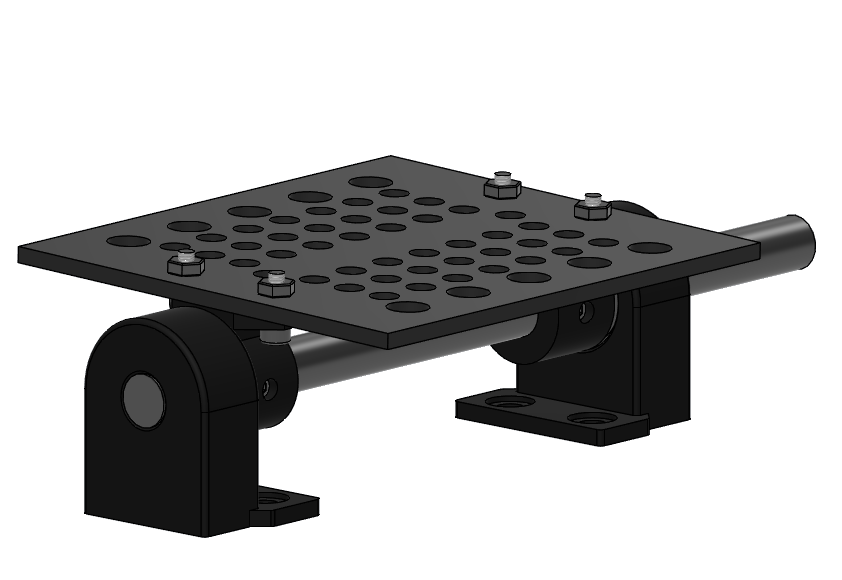
\includegraphics[width=\linewidth]{Recursos/Imagenes/ImagenesDisenoMecanico/SubsistemaOrientacionDisenhoA1.png}
	\end{minipage}\hfill
	\begin{minipage}{0.5\textwidth}
		\centering
		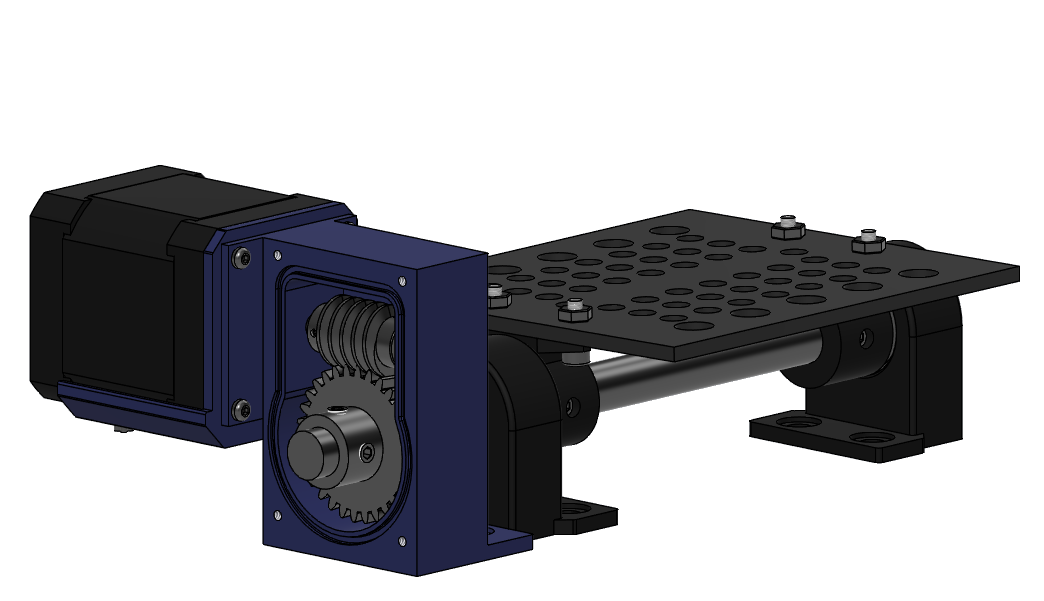
\includegraphics[width=\linewidth]{Recursos/Imagenes/ImagenesDisenoMecanico/SubsistemaOrientacionDisenhoA2.png}
	\end{minipage}
	\par\medskip

	\raggedright
	\footnotesize \textit{Nota.} Derecha, flechas rojas representan la transmisión de potencia desde el motor hacia el eje.
	\label{fig:SubsistemaOrientacionDisenhoA}
\end{figure}

\subsection{Planteamiento cinemático y estático}

\subsubsection{Perfil de movimiento}

La plataforma recorre el barrido de $-30^\circ$ a $+30^\circ$ con un perfil trapezoidal de velocidad: acelera durante un tiempo $t_a = f_a\, t_b$, se mueve a velocidad constante y desacelera durante el mismo $t_a$. La velocidad angular máxima y la aceleración angular son:

\begin{equation}\label{eq:perfil_tilt}
    \omega_{\text{máx}} = \frac{\Delta\theta}{t_b - t_a}, \qquad \ddot{\theta} = \frac{\omega_{\text{máx}}}{t_a}
\end{equation}

Con $t_b = 5.0\text{ s}$ y $f_a = 0.25$, se obtiene $\omega_{\text{máx}} = 0.2793\text{ rad/s}$ ($16.00^\circ/\text{s}$) y $\ddot{\theta} = 0.2234\text{ rad/s}^2$. Con la reducción de 30 a 1, el motor gira a un máximo de $80\text{ rpm}$.

\begin{figure}[H]
	\captionsetup{justification=raggedright, singlelinecheck=false, labelsep=none}
	\caption[Esquematización de movimiento del subsistema de orientación (izquierda) y diagrama de cuerpo libre (derecha).]{}
	\textit{Esquematización de movimiento del subsistema de orientación (izquierda) y diagrama de cuerpo libre del subsistema de orientación (derecha).} \par\medskip

	\begin{minipage}{0.5\textwidth}
		\centering
		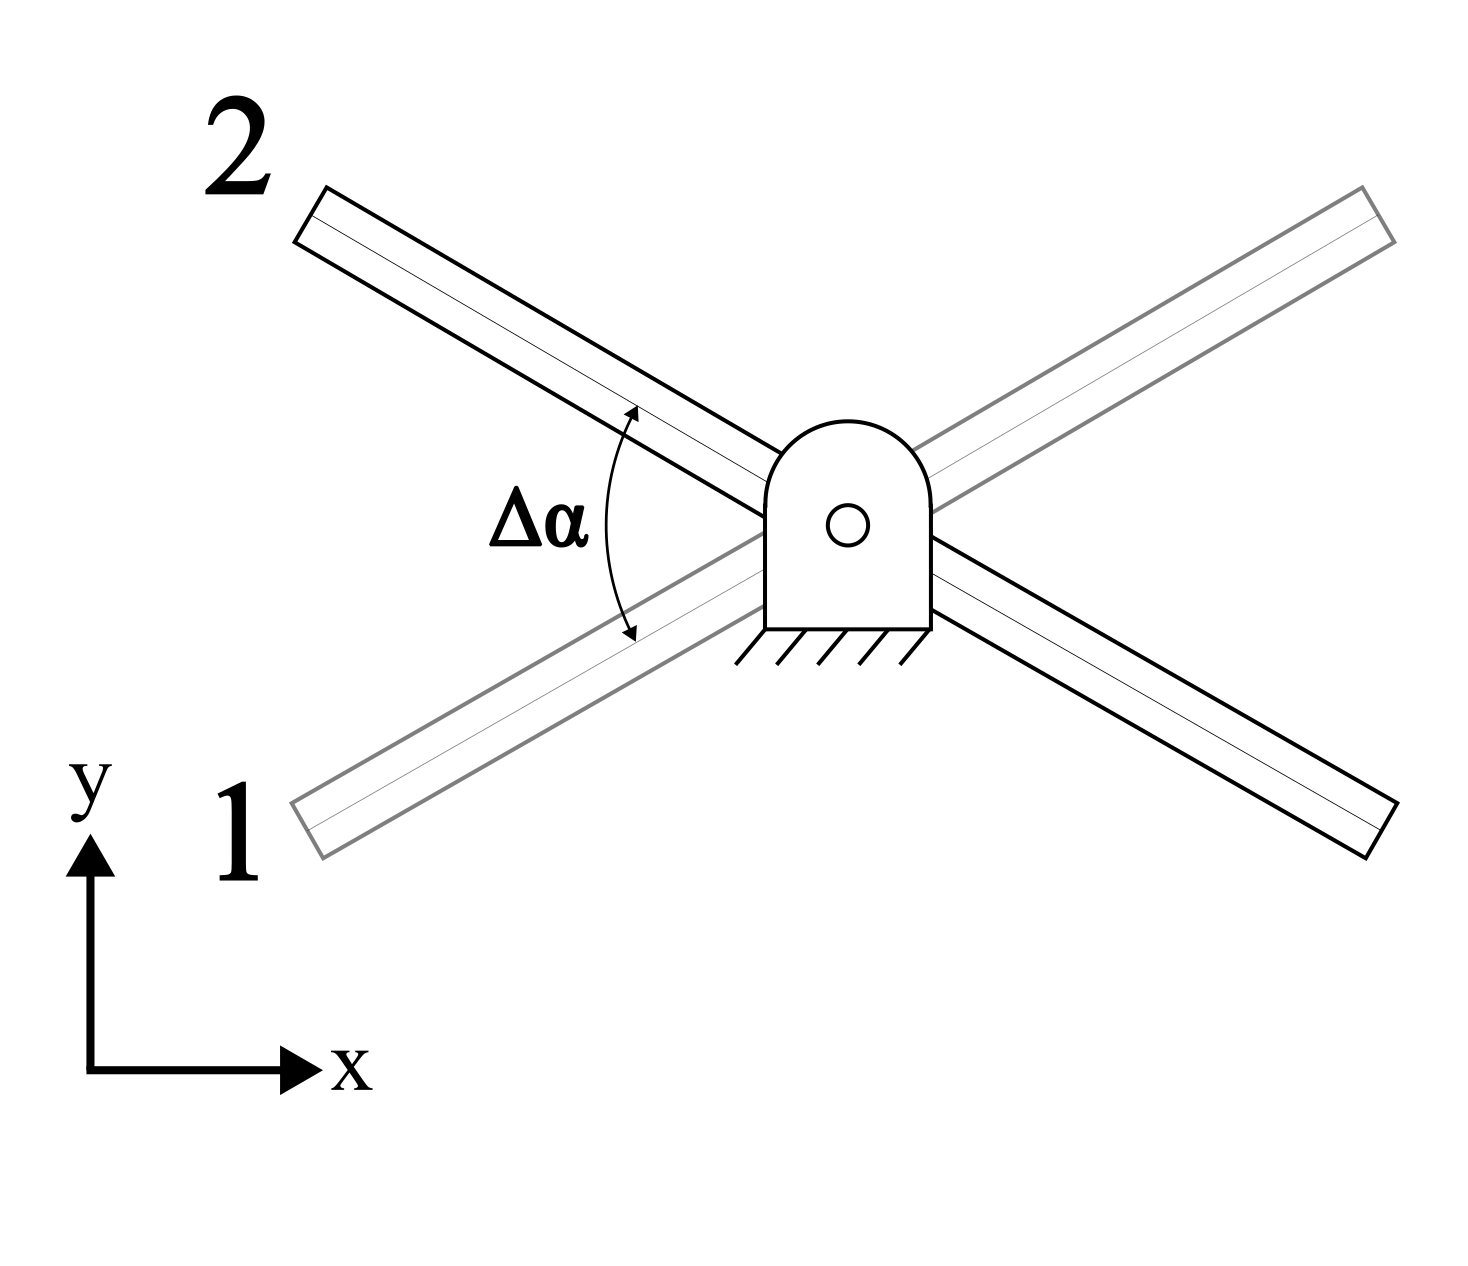
\includegraphics[width=\linewidth]{Recursos/Imagenes/ImagenesDisenoMecanico/Tilt_DCL_1.png}
	\end{minipage}\hfill
	\begin{minipage}{0.5\textwidth}
		\centering
		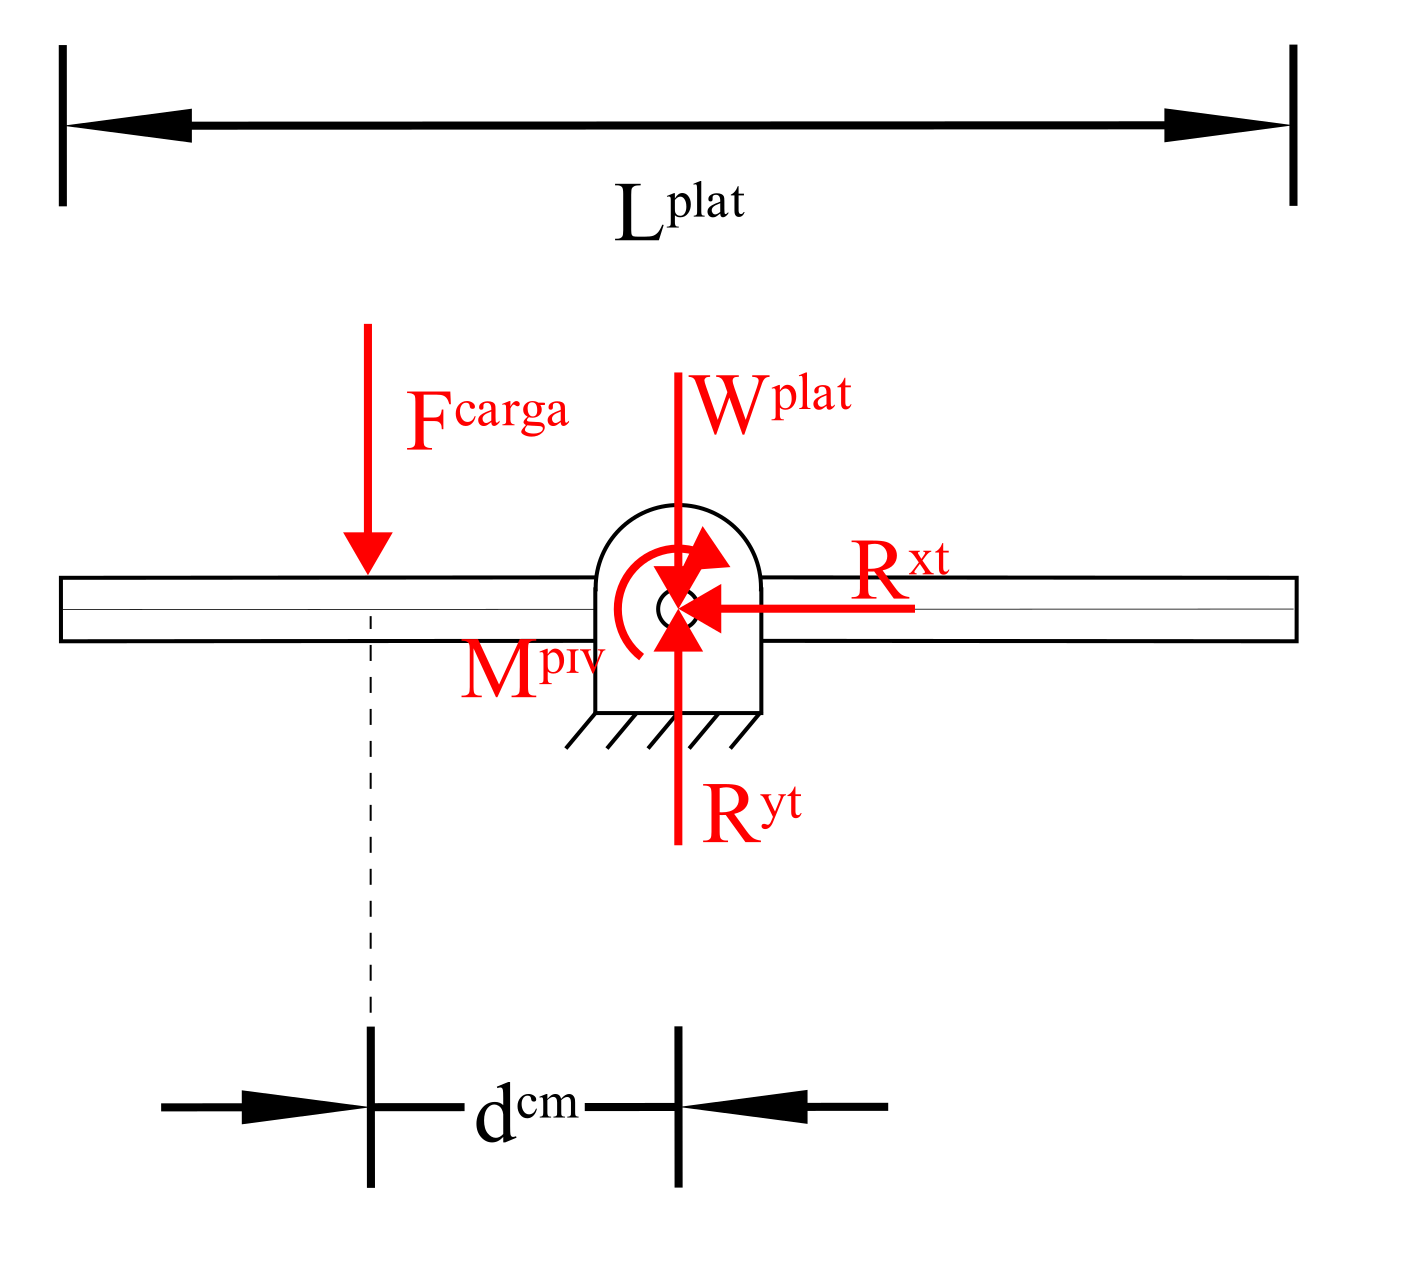
\includegraphics[width=\linewidth]{Recursos/Imagenes/ImagenesDisenoMecanico/Tilt_DCL_2.png}
	\end{minipage}
	\par\medskip

	\raggedright
	\footnotesize \textit{Nota.} Elaboración propia.
	\label{fig:DCLSubsistemaOrientacion}
\end{figure}

\subsubsection{Cargas sobre el eje de giro}

Según el diagrama de cuerpo libre de la Figura \ref{fig:DCLSubsistemaOrientacion}, el sensor y la plataforma generan momento gravitacional. El sensor lo genera por su excentricidad horizontal $d_{\text{cm}}$ y por la altura $z_s$ de su centro de masa sobre el eje; la plataforma, solo por la altura $z_p$. El momento gravitacional en función del ángulo es:
% RECORDATORIO: redibujar Tilt_DCL_2.png con la placa por encima del eje y los centros de masa del sensor y de la placa a las alturas z_s y z_p.

\begin{equation}\label{eq:Mpiv}
    M_{\text{piv}}(\theta) = g\left[m_{\text{carga}}\left(d_{\text{cm}} \cos\theta + z_s \sin\theta\right) + m_{\text{plat}}\, z_p \sin\theta\right]
\end{equation}

Como la excentricidad $d_{\text{cm}}$ puede estar a cualquier lado del eje, se toma el signo más desfavorable. Con él, el valor máximo ocurre en un extremo del barrido ($\theta = \pm 30^\circ$) y es $|M_{\text{piv}}| = 0.2595\text{ N}\cdot\text{m}$; en $\theta = 0^\circ$ vale $0.1226\text{ N}\cdot\text{m}$. El momento gravitacional cambia de signo dentro del barrido: con la excentricidad de diseño, en $\theta = \pm 21.8^\circ$, y con el sensor centrado, como en el modelo CAD, en $\theta = 0^\circ$.

La carga de viento se calcula con la norma NTE E.020 \citep{nte_e020}. La norma define la velocidad de diseño hasta $10\text{ m}$ de altura como la velocidad máxima de la zona según su mapa eólico, con un período de retorno de 50 años, y no menor de $75\text{ km/h}$. Como el robot no tiene un sitio de operación definido, se adopta el mínimo de $75\text{ km/h}$ para el cálculo, y como el sensor está a menos de $10\text{ m}$ de altura, se toma $V_h = V$. Para que el diseño no dependa del valor de cada zona, se repitió la cadena de cálculo con $130\text{ km/h}$, el mayor valor que se lee en el mapa eólico de la norma. Las verificaciones de resistencia y del motor (\textit{pull-out} y retención del motor, fluencia del eje, flexión del diente de la corona y prisioneros) mantienen un factor de seguridad de al menos $1.11$, y la primera en llegar a $1$ es el \textit{pull-out} del motor, a $139\text{ km/h}$. Por lo tanto, ninguno de estos componentes falla con la velocidad de diseño de cualquier zona del mapa. Este resultado usa como criterio un factor de seguridad de $1$: los factores mínimos de diseño ($3.0$ para el eje y $4$ para los prisioneros) y las demás verificaciones (fatiga, rodamientos, flechas, autobloqueo y error angular) no se evaluaron a $130\text{ km/h}$. La velocidad de diseño a la altura $h$ y la presión de viento son:

\begin{equation}\label{eq:viento_tilt}
    V_h = V \left(\frac{h}{10}\right)^{0.22}, \qquad P_h = f_r \cdot 0.005\, C\, V_h^2
\end{equation}

donde $V_h$ está en km/h y $P_h$ en kgf/m$^2$. El factor de forma $C = 1.5$ corresponde a elementos aislados con una dimensión corta en la dirección del viento, y el factor $f_r = 1.2$ se aplica a las estructuras Tipo 2, sensibles a ráfagas \citep{nte_e020}. La presión resultante es de $50.63\text{ kgf/m}^2$ ($496.5\text{ Pa}$). Sobre el área expuesta de $0.012\text{ m}^2$, la fuerza lateral es $F_v = 5.96\text{ N}$, y con el brazo de $60\text{ mm}$ genera un momento $M_v = 0.3575\text{ N}\cdot\text{m}$ sobre el eje. El área y el brazo son una envolvente: en el modelo CAD, el producto del área proyectada por la altura de su centroide es de $3.66 \times 10^{-4}\text{ m}^3$ con la plataforma nivelada y de $3.15 \times 10^{-4}\text{ m}^3$ a $\pm 30^\circ$, frente a $7.2 \times 10^{-4}\text{ m}^3$ de la envolvente, de modo que el momento de viento adoptado es cerca del doble del que resulta de la geometría. Aun así, el viento es la mayor de las cargas sobre el eje.

La fricción de los rodamientos del eje, $T_{\text{rod}} = 0.0201\text{ N}\cdot\text{m}$, se estima con el modelo simplificado de SKF \citep{skf2020bearings}. Este valor se estimó para rodamientos con sellos de contacto. Los rodamientos seleccionados tienen escudos metálicos, que no rozan el aro interior, por lo que su fricción es menor y el valor adoptado es conservador.

\subsubsection{Inercia y torque requerido}

La inercia respecto al eje de giro incluye la plataforma, el sensor (con el término de Steiner por su excentricidad), la corona y el propio eje:

\begin{equation}\label{eq:Jtotal_tilt}
    J_{\text{total}} = J_{\text{plat}} + J_{\text{carga}} + J_{\text{corona}} + J_{\text{eje}}
\end{equation}

Las inercias se obtienen del modelo CAD respecto al eje de giro, asignando a cada pieza la densidad de su material. La inercia del sensor es $J_{\text{carga}} = m_{\text{carga}}\left(k_s^2 + d_{\text{cm}}^2\right)$, donde $k_s = 61.3\text{ mm}$ es el radio de giro del sólido del sensor respecto al eje, que ya incluye la altura $z_s$ de su centro de masa; con densidad uniforme y la masa de diseño, $J_{\text{carga}} = 2.193 \times 10^{-3}\text{ kg}\cdot\text{m}^2$. La inercia de la placa y su tornillería del modelo CAD, escalada a la masa de diseño de $0.25\text{ kg}$, es $J_{\text{plat}} = 2.284 \times 10^{-4}\text{ kg}\cdot\text{m}^2$. El sensor aporta la mayor parte del total, seguido de la plataforma; la corona ($5.9 \times 10^{-6}$) y el eje ($1.3 \times 10^{-6}\text{ kg}\cdot\text{m}^2$) contribuyen de forma marginal. La inercia total es $J_{\text{total}} = 2.429 \times 10^{-3}\text{ kg}\cdot\text{m}^2$.

Como la transmisión se autobloquea, el motor siempre debe impulsar la carga, incluso cuando la gravedad o el viento actúan a favor del giro. Por ello, el torque en el eje de salida se calcula sumando los módulos de todos los términos:

\begin{equation}\label{eq:Tout_tilt}
    T_{\text{out}}(t) = \left|M_{\text{piv}}(\theta)\right| + M_v + T_{\text{rod}} + J_{\text{total}} \left|\ddot{\theta}(t)\right|
\end{equation}

El torque requerido en el motor divide el torque de salida por la relación de reducción y la eficiencia estática del engrane, y suma la aceleración de las masas del lado del motor (rotor, tornillo sin fin y acoplamiento):

\begin{equation}\label{eq:Tmotor_tilt}
    T_{\text{motor}}(t) = \frac{S\, T_{\text{out}}(t)}{i\, \eta_s} + S\, J_{\text{m}}\, i \left|\ddot{\theta}(t)\right|
\end{equation}

Se usa la eficiencia estática $\eta_s$ porque el caso crítico de un motor a pasos es el arranque desde el reposo, cuando la fricción del engrane es máxima. La fricción de los rodamientos queda dentro de $T_{\text{out}}$, y la fricción del engrane, dentro de $\eta_s$, de modo que ninguna se cuenta dos veces.

\subsection{Dimensionamiento de componentes}

\subsubsection{Transmisión de tornillo sin fin y corona}

El diámetro del tornillo sin fin es una decisión de diseño, ya que el juego se fabrica a medida. Con un diámetro exterior de $14.5\text{ mm}$, el diámetro de paso es $d_w = 12.5\text{ mm}$, lo que corresponde a un factor diametral $q = d_w/m = 12.5$. El ángulo de avance, el diámetro de paso de la corona y la distancia entre centros son:

\begin{equation}\label{eq:geom_sinfin}
    \lambda = \arctan\!\left(\frac{m\, Z_1}{d_w}\right) = 4.574^\circ, \qquad d_2 = m\, Z_2 = 30\text{ mm}, \qquad a = \frac{d_w + d_2}{2} = 21.25\text{ mm}
\end{equation}

La eficiencia directa (el sin fin impulsa a la corona) se calcula según \citet{Shigley11th}. La eficiencia inversa (la corona impulsa al sin fin) se obtiene de las mismas componentes de fuerza, invirtiendo el sentido de la fuerza de fricción:

\begin{equation}\label{eq:eta_sinfin}
    \eta = \frac{\cos\phi_n - \mu \tan\lambda}{\cos\phi_n + \mu \cot\lambda}, \qquad
    \eta_{\text{inv}} = \frac{\cos\phi_n - \mu \cot\lambda}{\cos\phi_n + \mu \tan\lambda}
\end{equation}

Con $\mu_s = 0.15$, la eficiencia estática es $\eta_s = 0.330$ y la eficiencia inversa es negativa ($\eta_{\text{inv}} = -0.983$), lo que confirma que el mecanismo se autobloquea en reposo. La condición equivalente, según KHK \citep{khk_gear_ref}, es que la fricción supere el límite $\mu_{\text{lím}} = \cos\phi_n \tan\lambda = 0.0752$; con $\mu_s = 0.15$, el margen de autobloqueo es de $2.00$. Como referencia, en movimiento la velocidad de deslizamiento es de $0.053\text{ m/s}$, la fricción dinámica según la correlación AGMA \citep{Shigley11th} es de $0.087$ y la eficiencia sube a $0.460$.

El margen de autobloqueo depende de la fricción real del contacto, que disminuye con la lubricación y la vibración de marcha. Con el valor dinámico de $0.087$ el margen baja a $1.16$, y por debajo de $\mu = 0.075$ el autobloqueo desaparece (ver la Tabla \ref{tab:sensibilidad_mu_tilt}). Por ello, la posición no se confía solo al autobloqueo: el driver mantiene una corriente de retención reducida en el motor y el lazo cerrado con el sensor inercial corrige cualquier deriva.

Las fuerzas en el engrane se calculan con el torque de salida máximo afectado por el factor $S$ \citep{Shigley11th}. La fuerza tangencial en la corona, que es igual al empuje axial sobre el sin fin, es de $55.26\text{ N}$; la fuerza tangencial en el sin fin, igual a la fuerza axial sobre la corona, es de $13.41\text{ N}$; y la fuerza radial de separación es de $20.44\text{ N}$. Los apoyos del tornillo sin fin deben resistir el empuje axial de $55.26\text{ N}$.
El eje del motor admite como máximo una carga axial dinámica de $10\text{ N}$ y una carga radial dinámica de $21\text{ N}$ a $20\text{ mm}$ de la cara de montaje \citep{stepperonline_17hs16}. El empuje axial del sin fin ($55.26\text{ N}$) y la resultante de sus fuerzas radial y tangencial ($\sqrt{20.44^2 + 13.41^2} = 24.4\text{ N}$) superan esos límites, por lo que el sin fin se apoya en dos rodamientos propios, del mismo tipo que los del eje basculante (MR2010A con escudos), y se une al motor mediante un acoplamiento que no transmite esfuerzos axiales ni radiales al eje del motor. Como cota superior, sin depender de la separación entre ellos, se supone que un solo rodamiento recibe toda la carga radial y todo el empuje axial: $P_0 = 0.6 \times 24.4 + 0.5 \times 55.26 = 42.3\text{ N}$, mayor que la carga radial, de modo que, con la capacidad estática de $792\text{ N}$ \citep{mr2010a_bearing}, el factor de seguridad estático es $S_0 = 18.7$.
El acoplamiento entre el motor y el sin fin es flexible, lo que reduce las cargas que una desalineación entre ambos ejes transmitiría al eje del motor, y se fija a ambos ejes, de $5\text{ mm}$, con prisioneros. El torque máximo en el motor, $0.0839\text{ N}\cdot\text{m}$, se transmite con un factor de seguridad de al menos $6.6$ aun con un solo prisionero del menor tamaño que considera \citet{Shigley11th} (n.º 0, $222\text{ N}$ de retención), por encima del mínimo de $4$ para cargas dinámicas. El empuje axial del sin fin debe tomarlo su rodamiento fijo axialmente y no el acoplamiento, para no cargar el eje del motor más allá de su límite axial de $10\text{ N}$.
La Figura \ref{fig:CorteSinFin} muestra el corte del tornillo sin fin con sus rodamientos y el acoplamiento con el motor.

\begin{figure}[H]
	\captionsetup{justification=raggedright, singlelinecheck=false, labelsep=none}
	\caption[Corte del tornillo sin fin, sus rodamientos y el acoplamiento con el motor.]{}
	\textit{Corte del tornillo sin fin, sus rodamientos y el acoplamiento con el motor.} \par\medskip

	\centering
	% PENDIENTE: crear la imagen Recursos/Imagenes/ImagenesDisenoMecanico/Tilt_SinFin_Corte.png (corte del sin fin, sus rodamientos y el acoplamiento) y reemplazar el placeholder.
	
\includegraphics[width=0.85\linewidth]{Recursos/Imagenes/Placeholder.png}
	\par\medskip

	\raggedright
	\footnotesize \textit{Nota.} Elaboración propia.
	\label{fig:CorteSinFin}
\end{figure}
El esfuerzo de flexión en los dientes de la corona se estima con la ecuación de Lewis adaptada a coronas de sin fin, $\sigma_a = W_{Gt}/(p_n F_e y)$ \citep{Shigley11th}, con el paso normal $p_n = \pi m \cos\lambda = 3.13\text{ mm}$, un ancho de cara $F_e = 10\text{ mm}$, igual al de la corona de referencia \citep{khk_pg1_30r1j8} y mayor que el mínimo de $2m\sqrt{q+1} + 1.5m = 8.85\text{ mm}$ que recomienda KHK \citep{khk_gear_ref}, y el factor de forma $y = 0.125$ para $\phi_n = 20^\circ$. Con la fuerza tangencial de $55.26\text{ N}$, $\sigma_a = 14.1\text{ MPa}$. El límite de fluencia del bronce SAE 660 es de $95\text{ MPa}$ fundido por centrifugación y de $140\text{ MPa}$ en colada continua \citep{metals4u_sae660}; con el menor, el factor de seguridad a la fluencia es de $6.7$. Esta verificación es estática; no evalúa el desgaste ni la fatiga de los dientes.
La flecha del sin fin se verifica con el método de la viga equivalente de AGMA 6022-D19, que la limita a $0.025\,p_x$ (en mm) para que el contacto no se desplace en exceso \citep{agma6022_2019}. Con el paso axial $p_x = \pi m = 3.14\text{ mm}$, la flecha admisible es de $0.0785\text{ mm}$. Con el diámetro de raíz del sin fin, $10.0\text{ mm}$, la carga de $24.4\text{ N}$ aplicada en el centro del vano, que es el caso más desfavorable, y $E = 206\,850\text{ N/mm}^2$, la flecha es $y = F l^3/(48 E I)$, y se mantiene dentro del límite para cualquier separación entre los apoyos del sin fin menor de $250\text{ mm}$, mucho mayor que la de la caja del sin fin.

La distancia entre centros del modelo CAD es de $21.25\text{ mm}$, igual a la de la Ecuación \ref{eq:geom_sinfin}. Con ella, la holgura entre la cresta del sin fin y el fondo de la corona y la holgura entre la cresta de la corona y el fondo del sin fin son de $0.25\text{ mm}$, iguales a la holgura de fondo normal de $0.25\,m$, que resulta de una altura de diente de $2.25\,m$ y un addendum de $1.00\,m$ \citep{khk_gear_ref}; para pasos axiales menores de $0.16\text{ in}$, las expresiones de \citet{Shigley11th} dan el mismo valor. La caja del sin fin se fabrica con esa medida nominal y con la tolerancia que exige el juego circunferencial de diseño.
% RECORDATORIO: llevar el ancho de cara de la corona a 10 mm en el CAD. El calculo del eje supone que el plano medio de la corona queda a 35.5 mm del rodamiento derecho; si se desplaza, actualizar P.a_cor en MC01 y volver a ejecutar las memorias.

\subsubsection{Eje basculante}

La Figura \ref{fig:SubsistemaOrientacionDisenhoA} muestra la disposición del eje. De izquierda a derecha se encuentran el rodamiento izquierdo, los dos soportes de la plataforma ubicados junto a cada rodamiento, el rodamiento derecho y, en voladizo fuera de los rodamientos, la corona y la chapa del sensor inercial. Según el modelo CAD, los dos rodamientos están separados $111\text{ mm}$; cada soporte de la plataforma está a $13\text{ mm}$ de su rodamiento, el plano medio de la corona a $35.5\text{ mm}$ por fuera del rodamiento derecho y la chapa del sensor inercial a $54.6\text{ mm}$.

El eje se modela como una viga simplemente apoyada en los rodamientos, con un voladizo a la derecha. Las cargas son:
\begin{itemize}
    \item la resultante de los pesos y el viento sobre la plataforma ($9.47\text{ N}$), repartida en partes iguales entre los dos soportes;
    \item la resultante de las fuerzas tangencial y radial de la corona, que son perpendiculares entre sí ($\sqrt{55.26^2 + 20.44^2} = 58.91\text{ N}$), más el peso de la corona ($0.52\text{ N}$), en el plano medio de la corona;
    \item el momento concentrado que produce la fuerza axial de la corona ($13.41\text{ N}$) al actuar sobre su radio de paso;
    \item el peso de la tarjeta del sensor inercial ($0.03\text{ N}$); la chapa, impresa en ABS, no se cuenta.
\end{itemize}
La carga de la plataforma y la de la corona actúan en planos distintos; se suman como si fueran colineales y del mismo sentido, lo que es conservador.

La carga de la plataforma entra cerca de los rodamientos y casi no flexiona el eje; la fuerza de engrane en voladizo es la que lo dimensiona. El rodamiento derecho soporta $85.03\text{ N}$, mientras que la reacción en el rodamiento izquierdo es de $-16.10\text{ N}$, es decir, actúa en sentido opuesto a las cargas. El momento flector máximo, de $2.3127\text{ N}\cdot\text{m}$, ocurre en el rodamiento derecho. El par de $0.8289\text{ N}\cdot\text{m}$ (torque de salida por el factor $S$) recorre el eje desde la corona hasta el soporte derecho de la plataforma, por lo que la sección crítica está en el rodamiento derecho, donde coinciden el momento flector máximo y el par.

Para el eje de acero AISI 1045 de $10\text{ mm}$, con un límite de fluencia de $310\text{ MPa}$ \citep{asm2002steels} y un factor de concentración de esfuerzos $K_t = 2.0$ por los asientos de los prisioneros, los esfuerzos en la sección crítica son:

\begin{equation}\label{eq:esfuerzos_eje_tilt}
    \sigma = K_t \frac{32\, M}{\pi d^3} = 47.11\text{ MPa}, \qquad
    \tau = \frac{16\, T}{\pi d^3} = 4.22\text{ MPa}, \qquad
    \sigma' = \sqrt{\sigma^2 + 3\tau^2} = 47.68\text{ MPa}
\end{equation}

El límite de fluencia de $310\text{ MPa}$ es conservador: \citet{Shigley11th} da $340\text{ MPa}$ para el AISI 1045 laminado en caliente y $530\text{ MPa}$ para el estirado en frío, que corresponde a la barra calibrada seleccionada. Con $310\text{ MPa}$, el factor de seguridad a la fluencia es de $6.50$ (con $530\text{ MPa}$ sería de $11.1$). Con un factor de seguridad de diseño de $3.0$, el diámetro mínimo según la energía de distorsión es de $7.73\text{ mm}$, por lo que el eje de $10\text{ mm}$ cumple. El cortante transversal máximo, $4V/3A$ \citep{Shigley11th}, calculado con la fuerza cortante del voladizo ($59.46\text{ N}$), es de $1.01\text{ MPa}$ y es despreciable.
El eje realiza un barrido de ida y vuelta cada $5$ minutos y recibe además las ráfagas de viento, por lo que se verifica para vida infinita, con el criterio ED-Goodman y todos los esfuerzos tratados como completamente alternantes \citep{Shigley11th}. Con criterios conservadores ($S_{ut} = 620\text{ MPa}$ del AISI 1045 laminado en caliente, factor de superficie de maquinado aunque la barra es rectificada, factor de tamaño de barra rotatoria, confiabilidad de $99\%$ y $K_f = K_t = 2.0$ en flexión y torsión), el límite de fatiga según la misma fuente es $S_e = 185\text{ MPa}$ y el esfuerzo alternante de Von Mises es de $49.3\text{ MPa}$, de modo que el factor de seguridad a fatiga es de $3.7$ y la vida del eje no está limitada por el número de ciclos.

Como la corona está en voladizo, la flecha del eje en la corona altera la distancia entre centros y el juego del engrane. Considerando solo las cargas del voladizo, porque las de la plataforma tienden a levantarlo, la flecha en la corona es de $0.0399\text{ mm}$, con $E = 207\text{ GPa}$ \citep{Shigley11th}. Se calcula con el caso de viga simplemente apoyada con carga en voladizo de \citet{Shigley11th}, más el efecto del momento de la fuerza axial obtenido por superposición. Este valor es menor que el admisible de $0.076\text{ mm}$ ($0.003\text{ in}$) que recomienda \citet{Shigley11th} para engranes de 20 a 50 dientes por pulgada, rango en el que está el módulo 1 ($25.4$ dientes por pulgada).

La misma fuente limita la pendiente del eje. En los rodamientos, la pendiente es de $0.00042\text{ rad}$ (izquierdo) y $0.00084\text{ rad}$ (derecho), dentro del rango de $0.001$ a $0.003\text{ rad}$ que admiten los rodamientos rígidos de bolas. En la corona, la pendiente es de $0.00128\text{ rad}$ ($4.4'$). Esa fuente solo da un límite para engranes rectos ($0.0005\text{ rad}$), y AGMA 6022-D19 no fija un límite de pendiente del eje de la corona. Como referencia se usa su tolerancia de angularidad de la caja: la mayoría de las transmisiones de tornillo sin fin admiten un ángulo entre ejes de $90^\circ \pm 5'$, con alguna variación del patrón de contacto \citep{agma6022_2019}. La pendiente de $4.4'$ está dentro de ese valor, pero se suma a la angularidad de los alojamientos de la caja, para la que quedan solo $0.6'$. Por ello, el patrón de contacto debe comprobarse en el prototipo con tinta azul, como indica la misma norma, en tres posiciones a $120^\circ$ de la corona \citep{agma6022_2019}.
En consecuencia, se especifica que el ángulo entre el eje del sin fin y el eje basculante, una vez montados, no se aparte de $90^\circ$ en más de $0.6'$, lo que equivale a una tolerancia de perpendicularidad de $0.017\text{ mm}$ por cada $100\text{ mm}$ de longitud del eje. Como los alojamientos del eje basculante y la caja del sin fin son piezas distintas, esta tolerancia se asegura en el montaje, con superficies de referencia comunes en la base, y se comprueba con el patrón de contacto.

El giro por torsión del tramo de $48.5\text{ mm}$ entre la corona y el soporte derecho de la plataforma, calculado con $G = 79.3\text{ GPa}$ \citep{Shigley11th} y con el torque de salida sin el factor $S$ porque se usa en el presupuesto de error, es de $0.0228^\circ$.

La corona, los soportes de la plataforma y la chapa del sensor se fijan al eje con dos prisioneros de punta copa por cubo, que asientan sobre planos mecanizados en el eje. En el modelo CAD, los prisioneros de la corona y de los soportes son M4. Como valor conservador se adopta la fuerza de retención de un prisionero n.º 4 (de menor diámetro que el M4), de $712\text{ N}$ ($160\text{ lbf}$), según \citet{Shigley11th}; con ella, cada cubo transmite un par de $7.12\text{ N}\cdot\text{m}$. Los factores de seguridad al deslizamiento son de $8.59$ frente al par y de $106.2$ frente a la fuerza axial de la corona, por encima del rango de $4$ a $8$ que la misma fuente recomienda para cargas dinámicas. Ese valor supone prisioneros de acero aleado contra un eje de acero, roscados en el cubo. La corona es de bronce, pero los soportes de la plataforma y la chapa del sensor inercial son de ABS, con los prisioneros roscados en insertos; en ellos, la fuerza de retención está limitada además por la retención del inserto en el ABS, que esa fuente no cubre.

En los soportes, el inserto limita la fuerza que el prisionero puede ejercer sobre el eje. Al apretar el prisionero, la reacción del eje empuja el inserto hacia afuera, en la dirección de extracción; es la condición de un tornillo que hace tope en el fondo, que la guía de diseño de SPIROL señala como causa de que el inserto se salga (\textit{jack-out}) \citep{spirol_inserts_guide}. Los insertos son PEM IPFC-M4 (de acero inoxidable, a presión, con brida), para los que el fabricante da en ABS una fuerza de extracción de $324\text{ N}$ y un par de giro de $2.35\text{ N}\cdot\text{m}$ \citep{pem_si_inserts}. Con la relación $T = K F d$ y $K = 0.2$ \citep{Shigley11th}, que la guía de SPIROL también usa con un coeficiente de fricción de $0.2$ \citep{spirol_inserts_guide}, el prisionero M4 alcanza esa fuerza con un par de apriete de solo $0.26\text{ N}\cdot\text{m}$, menor que el par de asiento de $0.56\text{ N}\cdot\text{m}$ ($5\text{ lbf}\cdot\text{in}$) con que \citet{Shigley11th} obtiene los $712\text{ N}$ de retención; en el prisionero n.º 4 ese par produce una fuerza de unos $990\text{ N}$. Por ello, en los soportes de ABS no puede alcanzarse esa retención. Si se supone que la retención es proporcional a la fuerza del prisionero, con la fuerza limitada a la de extracción del inserto resulta una retención de unos $232\text{ N}$ por prisionero, un par transmisible de $2.32\text{ N}\cdot\text{m}$ por soporte y un factor de seguridad de $2.8$ frente al par de $0.8289\text{ N}\cdot\text{m}$, menor que el rango de $4$ a $8$ recomendado para cargas dinámicas. Además, los datos del fabricante corresponden a ABS moldeado, y una pieza impresa en ABS puede tener menor resistencia: la guía de SPIROL indica que los agujeros moldeados rinden más que los taladrados, que el diámetro óptimo del alojamiento es de 2 a 3 veces el del inserto y que los plásticos pierden carga por fluencia lenta \citep{spirol_inserts_guide}. PennEngineering recomienda ensayar el inserto en cada aplicación \citep{pem_si_inserts}. Por lo tanto, la fijación de los soportes al eje debe verificarse en el prototipo midiendo el par al que el soporte desliza sobre el eje.

La Figura \ref{fig:CorteEjeBasculante} muestra el corte del eje basculante con sus rodamientos, los soportes de la plataforma, la corona y la chapa del sensor inercial.

\begin{figure}[H]
	\captionsetup{justification=raggedright, singlelinecheck=false, labelsep=none}
	\caption[Corte del eje basculante.]{}
	\textit{Corte del eje basculante.} \par\medskip

	\centering
	% PENDIENTE: crear la imagen Recursos/Imagenes/ImagenesDisenoMecanico/Tilt_Eje_Corte.png (corte del eje basculante) y reemplazar el placeholder.
	
\includegraphics[width=0.85\linewidth]{Recursos/Imagenes/Placeholder.png}
	\par\medskip

	\raggedright
	\footnotesize \textit{Nota.} Elaboración propia.
	\label{fig:CorteEjeBasculante}
\end{figure}

\subsubsection{Rodamientos del eje basculante}

El rodamiento derecho, junto a la corona, es el más cargado y además fija la posición axial del eje, por lo que recibe la fuerza axial de la corona de $13.41\text{ N}$; el rodamiento izquierdo es libre en dirección axial. La carga estática equivalente es $P_0 = 0.6\,F_r + 0.5\,F_a = 57.72\text{ N}$; como resulta menor que la carga radial, se toma $P_0 = F_r = 85.03\text{ N}$ \citep{skf2020bearings}. Con la capacidad estática de $792\text{ N}$ ($80.8\text{ kgf}$) del rodamiento MR2010A con escudos (ZZ) de $10\times20\times6\text{ mm}$ \citep{mr2010a_bearing}, el factor de seguridad estático es $S_0 = 9.32$. Como la reacción del rodamiento izquierdo cambia de sentido, su alojamiento debe retenerlo en ambas direcciones radiales.

\subsection{Selección de componentes}

\subsubsection{Selección del actuador de orientación}

El motor debe entregar el torque máximo de la Ecuación \ref{eq:Tmotor_tilt}, que es de $0.0839\text{ N}\cdot\text{m}$, a una velocidad de hasta $80\text{ rpm}$. Se comparan los motores NEMA 17 de la Tabla \ref{tab:comp_steppers}, todos con ángulo de paso de $1.8^\circ$.

\begin{center}
    \footnotesize
    \begin{xltabular}{\textwidth}{|p{3cm}|>{\centering\arraybackslash}X|>{\centering\arraybackslash}X|>{\centering\arraybackslash}X|>{\centering\arraybackslash}X|}
        \caption{Tabla comparativa de modelos de motor a pasos NEMA 17 evaluados\label{tab:comp_steppers}} \\
        \hline
        \rowcolor[HTML]{D9E1F2}
        Especificación Técnica & Opción A 17HS16-2004S1 & Opción B 17HS19-2004S1 & Opción C 17HS24-2104S & Opción D 42BYGHW811 \\ \hline
        \endfirsthead

        \multicolumn{5}{c}%
        {\tablename\ \thetable{} -- Continuación de la página anterior} \\
        \hline
        \rowcolor[HTML]{D9E1F2}
        Especificación Técnica & Opción A 17HS16-2004S1 & Opción B 17HS19-2004S1 & Opción C 17HS24-2104S & Opción D 42BYGHW811 \\ \hline
        \endhead

        \hline
        \endfoot

        \hline
        \endlastfoot

        Disponibilidad o Origen & Importación & Importación & Importación & Local o Importación \\ \hline
        Torque de Retención & $0.45\text{ N}\cdot\text{m}$ & $0.59\text{ N}\cdot\text{m}$ & $0.65\text{ N}\cdot\text{m}$ & $0.48\text{ N}\cdot\text{m}$ \\ \hline
        Ángulo de Paso & $1.8^\circ \pm 5\%$ & $1.8^\circ \pm 5\%$ & $1.8^\circ \pm 5\%$ & $1.8^\circ \pm 5\%$ \\ \hline
        Corriente Nominal por Fase & $2.0\text{ A}$ & $2.0\text{ A}$ & $2.1\text{ A}$ & $2.5\text{ A}$ \\ \hline
        Resistencia de Fase & $1.30\,\Omega$ & $1.40\,\Omega$ & $1.60\,\Omega$ & $1.20\,\Omega$ \\ \hline
        Inercia del Rotor & $54\text{ g}\cdot\text{cm}^2$ & $82\text{ g}\cdot\text{cm}^2$ & $115\text{ g}\cdot\text{cm}^2$ & $68\text{ g}\cdot\text{cm}^2$ \\ \hline
        Longitud del Cuerpo & $40\text{ mm}$ & $48\text{ mm}$ & $60\text{ mm}$ & $48\text{ mm}$ \\ \hline
        Masa Total & $0.31\text{ kg}$ & $0.40\text{ kg}$ \citep{skysmotor_17hs19} & $0.50\text{ kg}$ & $0.38\text{ kg}$ \\ \hline
        Diámetro de Eje & $\phi\,5.00\text{ mm}$ & $\phi\,5.00\text{ mm}$ & $\phi\,5.00\text{ mm}$ & $\phi\,5.00\text{ mm}$ \\ \hline
    \end{xltabular}
\end{center}

Las cuatro opciones superan con amplitud el torque requerido, por lo que el criterio de selección es reducir la masa sobre la plataforma elevada y la inercia del rotor. Se selecciona la Opción A, el motor 17HS16-2004S1, que es el más liviano ($0.31\text{ kg}$) y el de menor inercia de rotor. Su torque de retención a la corriente configurada de $1.40\text{ A}$ es de $0.315\text{ N}\cdot\text{m}$, lo que da un factor de seguridad de $3.75$.
% Masa (310 g), longitud (40 mm) y resistencia (1.3 ohm) del 17HS16: pagina del fabricante (stepperonline_17hs16). La hoja de datos actual deja en blanco la inercia del rotor; los 54 g cm^2 vienen de la version de 2020 de la hoja de datos.

La verificación determinante es frente al torque de extracción (\textit{pull-out}). La curva del fabricante \citep{stepperonline_17hs16} se midió con un driver DM542T a $24\text{ V}$, $2.05\text{ A}$ de pico y $2000$ pulsos por vuelta. Entre $0$ y $90\text{ rpm}$, el motor entrega $0.36\text{ N}\cdot\text{m}$ a $30$ y a $90\text{ rpm}$, pero cae a $0.29\text{ N}\cdot\text{m}$ a $60\text{ rpm}$ por resonancia. Como el motor arranca y acelera hasta $80\text{ rpm}$, pasa por esa velocidad, por lo que se toma $0.29\text{ N}\cdot\text{m}$ como el torque disponible en todo el rango. Escalado linealmente con la corriente, lo que es válido a baja velocidad, el torque disponible con los $1.40\text{ A}$ de pico configurados es de $0.29 \times 1.40/2.05 = 0.198\text{ N}\cdot\text{m}$, y el factor de seguridad frente al \textit{pull-out} es de $2.36$. Este valor supone que el driver del robot entrega esa corriente y una tensión de alimentación de al menos $24\text{ V}$, como en el ensayo del fabricante; la selección del driver no forma parte de este capítulo.

\subsubsection{Fabricación y materiales de la transmisión}

El tornillo sin fin y la corona se fabrican en torno CNC. El tornillo sin fin es de acero AISI 1045 sin tratamiento térmico, con los flancos pulidos. La corona es de bronce al plomo SAE 660 (UNS C93200), elegido por su maquinabilidad y su buen comportamiento al deslizamiento contra acero \citep{asm1990nonferrous}. Esta combinación sigue la práctica habitual en transmisiones de tornillo sin fin: el elemento más duro es el sin fin y el desgaste se concentra en la corona. La carga tangencial de $55.26\text{ N}$ y la velocidad de deslizamiento de $0.053\text{ m/s}$ son bajas, lo que justifica prescindir del tratamiento térmico del sin fin. El conjunto opera lubricado con grasa dentro de una caja sellada, con retenes en el paso del eje, para protegerlo del polvo abrasivo.

El juego circunferencial de diseño, $j_t = 0.28\text{ mm}$, se toma de coronas comerciales de módulo 1 y 30 dientes, cuyo juego varía entre $0$ y $0.28\text{ mm}$ en grado de precisión KHK W 002 grado 5 \citep{khk_pg1_30r1j8}. Este valor debe respetarse en las tolerancias de fabricación de los dientes y de la distancia entre centros.

\subsubsection{Selección de rodamientos}

Se seleccionan rodamientos rígidos de bolas MR2010A de $10\times20\times6\text{ mm}$, de acero al cromo, con escudos metálicos en ambos lados (ZZ) \citep{mr2010a_bearing}, dos para el eje basculante y dos para el tornillo sin fin. Su capacidad estática supera con amplitud la carga del rodamiento más exigido, como se mostró en la verificación anterior. Los escudos no rozan el aro interior, por lo que su fricción es baja, pero protegen menos contra el polvo que los sellos de contacto; por ello, los alojamientos deben limitar la entrada de polvo a los rodamientos. Esta medida no pertenece a las series ISO normalizadas, por lo que se debe confirmar su disponibilidad con el proveedor.

\subsubsection{Selección del eje basculante}

Se selecciona una barra de acero calibrado AISI 1045 de $10\text{ mm}$ de diámetro con acabado rectificado, con planos mecanizados en los asientos de los prisioneros. El diámetro mínimo por resistencia es de $7.73\text{ mm}$; el diámetro de $10\text{ mm}$ se adopta por estandarización con el diámetro interior de los rodamientos y para limitar la flecha en la corona.

\subsubsection{Soportes, bridas y elementos de fijación}

Para la base estructural se utilizan perfiles de aluminio extruido V-Slot 2040 de $20\times40\text{ mm}$, ensamblados mediante escuadras de fundición de $90^\circ$. El acoplamiento de los motores y sensores se realiza con placas de aluminio 6061-T6 de $3\text{ mm}$ de espesor mecanizadas por control numérico. Todo el ensamble se asegura con tornillería de acero inoxidable de grado A2-70 y tuercas tipo T corredizas para garantizar la resistencia a la intemperie.


\subsection{Simulación y validación}

Las ecuaciones de las secciones anteriores se implementaron en un modelo de cálculo en MATLAB que evalúa el subsistema a lo largo de toda la trayectoria. El modelo recibe los datos de la Tabla \ref{tab:parametros_diseno_tilt} y las dimensiones del modelo CAD, y calcula:
\begin{itemize}
    \item el perfil de movimiento;
    \item las cargas y el torque en el motor en cada instante;
    \item la eficiencia y el autobloqueo de la transmisión;
    \item las fuerzas del engrane;
    \item los diagramas de esfuerzos del eje;
    \item la verificación de los rodamientos y los prisioneros;
    \item el presupuesto de error angular.
\end{itemize}
También analiza la sensibilidad de los resultados al coeficiente de fricción. El modelo está organizado como memorias de cálculo numeradas de MC-01 a MC-16, una por componente o verificación, que se ejecutan en orden desde MC-00 y generan un reporte con los datos, las hipótesis, los resultados y el estado de cada verificación.

\subsubsection{Torque a lo largo de la trayectoria}
% Figuras generadas por MC07_torque_trayectoria.m y MC09_eje_basculante.m (memorias de calculo MC-00 a MC-16).

La Figura \ref{fig:Torques_Tilt} muestra el momento gravitacional, el torque en el eje de salida y el torque requerido en el motor a lo largo del barrido. Con el signo más desfavorable de la excentricidad, el módulo del momento gravitacional es máximo en un extremo del barrido y se anula en $\theta = 21.8^\circ$ del lado opuesto. El momento de viento se suma de forma constante, por lo que el torque de salida alcanza su máximo de $0.6376\text{ N}\cdot\text{m}$ en el extremo $\theta = -30^\circ$, al arrancar desde el reposo ($t = 0$). Ese punto coincide con el arranque, en el que la fricción del engrane es la estática, de modo que el uso de $\eta_s$ corresponde físicamente al caso crítico. El término inercial en las fases de aceleración es de apenas $5.4 \times 10^{-4}\text{ N}\cdot\text{m}$, es decir, el torque está dominado por las cargas estáticas y no por la dinámica del movimiento.

El torque máximo en el motor es de $0.0839\text{ N}\cdot\text{m}$ con la eficiencia estática y de $0.0602\text{ N}\cdot\text{m}$ con la eficiencia dinámica. En toda la trayectoria, ambas curvas se mantienen por debajo del torque de retención ($0.315\text{ N}\cdot\text{m}$) y del torque de \textit{pull-out} ($0.198\text{ N}\cdot\text{m}$) a la corriente configurada.

\begin{figure}[H]
	\captionsetup{justification=raggedright, singlelinecheck=false, labelsep=none}
	\caption[Torque en el eje de salida y en el motor a lo largo del barrido angular.]{}
	\textit{Torque en el eje de salida y en el motor a lo largo del barrido angular.} \par\medskip

	\centering
	% PENDIENTE: compilar y colocar la figura actualizada Tilt_Torques_MATLAB.png (generada por MC07) en Recursos/Imagenes/ImagenesDisenoMecanico/ y reemplazar el placeholder.
	
\includegraphics[width=0.85\linewidth]{Recursos/Imagenes/Placeholder.png}
	\par\medskip

	\raggedright
	\footnotesize \textit{Nota.} Elaboración propia en MATLAB.
	\label{fig:Torques_Tilt}
\end{figure}

\subsubsection{Esfuerzos en el eje basculante}

La Figura \ref{fig:Eje_Tilt} muestra los diagramas de momento flector y torsor del eje. Como la reacción del rodamiento izquierdo es opuesta a las cargas, el momento flector crece casi linealmente entre los rodamientos, desde cero en el izquierdo hasta su máximo de $2.3127\text{ N}\cdot\text{m}$ en el derecho; la carga de la plataforma, que entra junto a los rodamientos, apenas cambia la pendiente del diagrama. En el voladizo, el momento disminuye hasta el valor del par de la fuerza axial en la corona y se anula más allá de ella. El momento torsor de $0.8289\text{ N}\cdot\text{m}$ actúa solo en el tramo entre la corona y el soporte derecho de la plataforma. Ambos diagramas confirman que la sección crítica es el rodamiento derecho.

\begin{figure}[H]
	\captionsetup{justification=raggedright, singlelinecheck=false, labelsep=none}
	\caption[Diagramas de momento flector y momento torsor en el eje basculante.]{}
	\textit{Diagramas de momento flector y momento torsor en el eje basculante.} \par\medskip

	\centering
	% PENDIENTE: compilar y colocar la figura actualizada Tilt_Eje_MATLAB.png (generada por MC09) en Recursos/Imagenes/ImagenesDisenoMecanico/ y reemplazar el placeholder.
	
\includegraphics[width=0.85\linewidth]{Recursos/Imagenes/Placeholder.png}
	\par\medskip

	\raggedright
	\footnotesize \textit{Nota.} Posición medida desde el centro del rodamiento izquierdo. Elaboración propia en MATLAB.
	\label{fig:Eje_Tilt}
\end{figure}

\subsubsection{Sensibilidad al coeficiente de fricción}

El coeficiente de fricción del contacto entre el sin fin y la corona es el parámetro más incierto del modelo y afecta en sentidos opuestos a dos verificaciones: una fricción alta reduce la eficiencia y aumenta el torque requerido, mientras que una fricción baja reduce el margen de autobloqueo. La Tabla \ref{tab:sensibilidad_mu_tilt} muestra ambos efectos.

\begin{center}
    \footnotesize
    \begin{xltabular}{\textwidth}{|>{\centering\arraybackslash}X|>{\centering\arraybackslash}X|>{\centering\arraybackslash}X|>{\centering\arraybackslash}X|>{\centering\arraybackslash}X|}
        \caption{Sensibilidad de la transmisión al coeficiente de fricción\label{tab:sensibilidad_mu_tilt}} \\
        \hline
        \rowcolor[HTML]{D9E1F2}
        $\mu$ & $\eta$ & Margen de autobloqueo $\mu/\mu_{\text{lím}}$ & $T_{\text{motor}}$ [N$\cdot$m] & FS frente a \textit{pull-out} \\ \hline
        \endfirsthead

        \multicolumn{5}{c}%
        {\tablename\ \thetable{} -- Continuación de la página anterior} \\
        \hline
        \rowcolor[HTML]{D9E1F2}
        $\mu$ & $\eta$ & Margen de autobloqueo $\mu/\mu_{\text{lím}}$ & $T_{\text{motor}}$ [N$\cdot$m] & FS frente a \textit{pull-out} \\ \hline
        \endhead

        \hline
        \endfoot

        \hline
        \endlastfoot

        $0.050$ & $0.598$ & $0.67$ (sin autobloqueo) & $0.0463$ & $4.28$ \\ \hline
        $0.075$ & $0.497$ & $1.00$ (límite) & $0.0556$ & $3.56$ \\ \hline
        $0.087$ (dinámico) & $0.460$ & $1.16$ & $0.0601$ & $3.29$ \\ \hline
        $0.100$ & $0.425$ & $1.33$ & $0.0650$ & $3.05$ \\ \hline
        $0.150$ (diseño) & $0.330$ & $2.00$ & $0.0839$ & $2.36$ \\ \hline
        $0.200$ & $0.269$ & $2.66$ & $0.1029$ & $1.92$ \\ \hline
    \end{xltabular}
\end{center}

En todo el rango analizado, el factor de seguridad del motor frente al \textit{pull-out} se mantiene por encima de $1.9$, por lo que el actuador es adecuado aunque la fricción sea mayor que la de diseño. En cambio, el autobloqueo solo está garantizado en reposo; en movimiento o bajo vibración, el margen puede acercarse a $1$. Este resultado justifica mantener la corriente de retención en el driver y cerrar el lazo de posición con el sensor inercial.

\subsubsection{Presupuesto de error angular}

La resolución del motor no equivale a la precisión del sistema. Con la reducción de 30 a 1, el motor alcanza una resolución de $0.06^\circ$ a paso completo y de $0.00375^\circ$ con 16 micropasos, pero el juego del engrane de $0.28\text{ mm}$ sobre el radio de paso de la corona equivale a un error de $1.070^\circ$. La Tabla \ref{tab:error_angular_tilt} compara la operación en lazo abierto con la operación en lazo cerrado.

\begin{center}
    \footnotesize
    \begin{xltabular}{\textwidth}{|X|>{\centering\arraybackslash}p{3cm}|>{\centering\arraybackslash}p{3cm}|}
        \caption{Presupuesto de error angular de inclinación\label{tab:error_angular_tilt}} \\
        \hline
        \rowcolor[HTML]{D9E1F2}
        Fuente de error & Lazo abierto [$^\circ$] & Lazo cerrado [$^\circ$] \\ \hline
        \endfirsthead

        \multicolumn{3}{c}%
        {\tablename\ \thetable{} -- Continuación de la página anterior} \\
        \hline
        \rowcolor[HTML]{D9E1F2}
        Fuente de error & Lazo abierto [$^\circ$] & Lazo cerrado [$^\circ$] \\ \hline
        \endhead

        \hline
        \endfoot

        \hline
        \endlastfoot

        Juego del engrane & $1.070$ & Compensado \\ \hline
        Resolución del actuador & $0.060$ & $0.00375$ \\ \hline
        Exactitud del sensor inercial & -- & $0.100$ \\ \hline
        Montaje del sensor y de los soportes & $0.200$ & $0.200$ \\ \hline
        Holgura de los rodamientos & $0.050$ & $0.050$ \\ \hline
        Giro por torsión del eje & -- & $0.0228$ \\ \hline
        \textbf{Suma lineal} & $\mathbf{1.380}$ & $\mathbf{0.377}$ \\ \hline
        \textbf{Suma cuadrática (RSS)} & $1.091$ & $0.230$ \\ \hline
        \textbf{Tolerancia IEC 61724-1, Clase A} & $0.5$ & $0.5$ \\ \hline
    \end{xltabular}
\end{center}

En lazo abierto, solo el juego del engrane ya supera la tolerancia de $0.5^\circ$, por lo que el lazo cerrado es indispensable. El sensor inercial está montado en una chapa solidaria al eje, por fuera de la corona; al medir el ángulo del eje, compensa el juego del engrane. Esta compensación solo es válida mientras el momento externo sobre el eje no cambie de signo durante la medición, porque la corona queda retenida contra el flanco del sin fin sobre el que se apoya. Si el momento cambia de signo, la corona cruza el juego, de hasta $1.07^\circ$, sin que el motor gire.

Con el sensor equilibrado sobre el eje, como en el modelo CAD, el peso del sensor y de la placa retiene la corona con un momento $g\,(m_{\text{carga}} z_s + m_{p} z_p)\sin\theta$, que crece con la inclinación y se anula en $\theta = 0^\circ$; aquí $m_p = 0.066\text{ kg}$ es la masa de la placa y su tornillería, sin los soportes de ABS, lo que da un valor bajo del momento de retención. Una ráfaga en sentido opuesto cruza el juego cuando su momento supera ese valor. Con la expresión de presión de la NTE E.020 sin el factor de ráfaga, porque el límite se expresa directamente como la ráfaga máxima, y con el área y el brazo de la envolvente, sin contar la fricción de los rodamientos, la ráfaga máxima admisible para la masa de diseño del sensor es de $21\text{ km/h}$ a $|\theta| = 5^\circ$, $33\text{ km/h}$ a $12^\circ$ y $51\text{ km/h}$ a $30^\circ$. Por ello, se establece como condición de operación que las mediciones solo son válidas con ráfagas de hasta $33\text{ km/h}$ para $|\theta| \geq 12^\circ$ y de hasta $21\text{ km/h}$ para $5^\circ \leq |\theta| < 12^\circ$; para $|\theta| < 5^\circ$ no se garantiza la tolerancia de inclinación. Estos límites dependen de la masa del sensor instalado: un sensor más liviano retiene menos la corona, y con el EKO MS-80 ($0.35\text{ kg}$) bajan a $28$ y $18\text{ km/h}$. También suponen que el sensor queda equilibrado sobre el eje; una excentricidad horizontal reduce el momento de retención a un lado del barrido, por lo que el equilibrio debe verificarse al montar el sensor.

Como referencia, en la planta solar Majes 20T (Arequipa), la velocidad media diaria del viento registrada entre 2016 y 2019 no superó $2.7\text{ m/s}$ ($9.7\text{ km/h}$) en 1394 días con datos \citep{gts_majes_2020}. Son medias diarias, por lo que no indican la frecuencia de ráfagas superiores a los límites anteriores, pero muestran que el sitio es de viento bajo.

El lazo no detecta los errores entre el eje y la plataforma, es decir, el giro por torsión y el montaje de los soportes y del sensor, por lo que estos se mantienen en el presupuesto. La hoja de datos del MPU-6050 no especifica una exactitud angular; especifica valores típicos de tolerancia del factor de escala de $\pm 3\%$ y de sensibilidad cruzada de $\pm 2\%$ \citep{invensense_mpu6050}. Si solo se calibra la desviación (\textit{offset}), una diferencia de escala $e$ entre los ejes Y y Z produce un error de alabeo de aproximadamente $e \sin\theta \cos\theta$, que a $30^\circ$ y con $e = 3\%$ es de $0.74^\circ$ y supera por sí solo la tolerancia. Por ello, el valor de $0.1^\circ$ de la Tabla \ref{tab:error_angular_tilt} exige calibrar el sensor en seis posiciones (desviación, escala y desalineación de ejes) y verificarlo frente a un inclinómetro de referencia. La temperatura también afecta la medición: la misma hoja de datos da una variación típica de la salida a cero $g$ de $\pm 35\text{ mg}$ en los ejes X e Y entre $0$ y $70^\circ\text{C}$, equivalente a unos $2^\circ$ de inclinación, y una variación de la sensibilidad de $\pm 0.02\%/^\circ\text{C}$ \citep{invensense_mpu6050}. Como el robot opera a la intemperie, la lectura del sensor inercial se compensa por temperatura con el sensor de temperatura integrado en el MPU-6050: durante la calibración se caracterizan la desviación y la sensibilidad a varias temperaturas, y el programa las corrige en cada medición. Con esta compensación, la deriva por temperatura no se incluye en el presupuesto de error, cuyo término de $0.1^\circ$ corresponde al sensor calibrado y compensado.
Con la suma lineal, que es el criterio más conservador, el error en lazo cerrado es de $0.377^\circ$, por debajo de la tolerancia de $0.5^\circ$, siempre que se cumplan la calibración descrita y la condición de operación de viento.

\subsubsection{Resumen de resultados}

La Tabla \ref{tab:resultados_tilt} resume las verificaciones del subsistema.

\begin{center}
    \footnotesize
    \begin{xltabular}{\textwidth}{|X|>{\centering\arraybackslash}p{2.6cm}|>{\centering\arraybackslash}p{2.6cm}|>{\centering\arraybackslash}p{1.8cm}|}
        \caption{Resumen de verificaciones del subsistema de orientación\label{tab:resultados_tilt}} \\
        \hline
        \rowcolor[HTML]{D9E1F2}
        Verificación & Resultado & Criterio & Estado \\ \hline
        \endfirsthead

        \multicolumn{4}{c}%
        {\tablename\ \thetable{} -- Continuación de la página anterior} \\
        \hline
        \rowcolor[HTML]{D9E1F2}
        Verificación & Resultado & Criterio & Estado \\ \hline
        \endhead

        \hline
        \endfoot

        \hline
        \endlastfoot

        Torque del motor frente a \textit{pull-out} & FS $= 2.36$ & FS $\geq 1$ & Cumple \\ \hline
        Torque del motor frente a retención & FS $= 3.75$ & FS $\geq 1$ & Cumple \\ \hline
        Autobloqueo en reposo ($\mu_s = 0.15$) & $\eta_{\text{inv}} = -0.983$ & $\eta_{\text{inv}} < 0$ & Cumple \\ \hline
        Flexión del diente de la corona (estática) & FS $= 6.7$ & FS $\geq 1$ & Cumple \\ \hline
        Holgura de fondo del engrane & $0.25\text{ mm}$ & $\geq 0.25\text{ mm}$ & Cumple \\ \hline
        Resistencia del eje a la fluencia & FS $= 6.50$ & FS $\geq 3.0$ & Cumple \\ \hline
        Fatiga del eje (vida infinita) & FS $= 3.7$ & FS $\geq 1$ & Cumple \\ \hline
        Flecha del eje en la corona & $0.0399\text{ mm}$ & $\leq 0.076\text{ mm}$ & Cumple \\ \hline
        Pendiente del eje en los rodamientos & $0.00084\text{ rad}$ & $\leq 0.001\text{ rad}$ & Cumple \\ \hline
        Pendiente del eje en la corona & $4.4'$ & $\leq 5'$ (AGMA 6022) & Cumple con angularidad de montaje $\leq 0.6'$ \\ \hline
        Rodamiento más cargado del eje basculante & $S_0 = 9.32$ & $S_0 \geq 1$ & Cumple \\ \hline
        Rodamientos del sin fin (cota superior) & $S_0 = 18.7$ & $S_0 \geq 1$ & Cumple \\ \hline
        Resistencia y motor con viento de $130\text{ km/h}$ (máximo del mapa eólico) & FS mín. $= 1.11$ & FS $\geq 1$ (sin margen de diseño) & Cumple \\ \hline
        Flecha del sin fin & vano $\leq 250\text{ mm}$ & $y \leq 0.025\,p_x$ & Cumple \\ \hline
        Prisioneros del acople motor--sin fin (par) & FS $\geq 6.6$ & FS $\geq 4$ & Cumple \\ \hline
        Prisioneros de la corona, de bronce (par / fuerza axial) & FS $= 8.59$ / $106.2$ & FS $\geq 4$ & Cumple \\ \hline
        Prisioneros de los soportes, en insertos en ABS (par) & FS $\approx 2.8$ (estimado) & FS $\geq 4$ & No cumple; verificar en prototipo \\ \hline
        Error angular en lazo cerrado & $0.377^\circ$ & $\leq 0.5^\circ$ & Cumple con calibración y límite de viento \\ \hline
    \end{xltabular}
\end{center}

El modelo de cálculo tiene limitaciones que deben considerarse al interpretar estos resultados:
\begin{itemize}
    \item supone cuerpos rígidos, salvo para la flecha y la torsión del eje;
    \item suma las cargas como colineales;
    \item adopta valores supuestos para la fricción, el juego del engrane y la exactitud del sensor inercial;
    \item calcula la inercia del sensor con densidad uniforme sobre su sólido del modelo CAD, con el centro de masa en su centro geométrico;
    \item no cuenta la masa de las piezas impresas en ABS.
\end{itemize}
Estos valores deben confirmarse en el prototipo midiendo el torque de arranque, el juego del engrane ensamblado y el error de inclinación frente a un inclinómetro de referencia.

\end{document}